%%% Hlavní soubor. Zde se definují základní parametry a odkazuje se na ostatní části. %%%

%% Verze pro jednostranný tisk:
% Okraje: levý 40mm, pravý 25mm, horní a dolní 25mm
% (ale pozor, LaTeX si sám přidává 1in)
\documentclass[a4paper,oneside,12p]{report}
%\documentclass[a4paper,oneside,12p,twoside]{report}
\setlength\textwidth{145mm}
\setlength\textheight{237mm}
%\setlength\oddsidemargin{00mm}
\setlength\oddsidemargin{15mm}
\setlength\evensidemargin{15mm}
\let\openright=\clearpage


%% Vytváříme PDF/A-2u
\usepackage[a-2u]{pdfx}

%% Přepneme na českou sazbu a fonty Latin Modern
\usepackage[czech]{babel}
\usepackage{lmodern}
\usepackage[T1]{fontenc}
\usepackage{textcomp}

%% Použité kódování znaků: obvykle latin2, cp1250 nebo utf8:
\usepackage[utf8]{inputenc}

%%% Další užitečné balíčky (jsou součástí běžných distribucí LaTeXu)
\usepackage{amsmath}        % rozšíření pro sazbu matematiky
\usepackage{amsfonts}       % matematické fonty
\usepackage{amsthm}         % sazba vět, definic apod.
\usepackage{bbding}         % balíček s nejrůznějšími symboly
			    % (čtverečky, hvězdičky, tužtičky, nůžtičky, ...)
\usepackage{bm}             % tučné symboly (příkaz \bm)
\usepackage{graphicx}       % vkládání obrázků
\usepackage{fancyhdr}		% možnost slylizovat záhlaví
\usepackage{fancyvrb}       % vylepšené prostředí pro strojové písmo
\usepackage{indentfirst}    % zavede odsazení 1. odstavce kapitoly
\usepackage{natbib}         % zajištuje možnost odkazovat na literaturu
			    % stylem AUTOR (ROK), resp. AUTOR [ČÍSLO]
\usepackage[nottoc]{tocbibind} % zajistí přidání seznamu literatury,
                            % obrázků a tabulek do obsahu
\usepackage{icomma}         % inteligetní čárka v matematickém módu
\usepackage{dcolumn}        % lepší zarovnání sloupců v tabulkách
\usepackage{booktabs}       % lepší vodorovné linky v tabulkách
\usepackage{paralist}       % lepší enumerate a itemize
\usepackage{listings}		% vkládání kódu
\usepackage{caption}		% popisky
\usepackage{dirtree}		% strom souborů

\usepackage{color}
\definecolor{pblue}{rgb}{0.13,0.13,1}
\definecolor{pgreen}{rgb}{0,0.5,0}
\definecolor{pred}{rgb}{0.9,0,0}
\definecolor{pgrey}{rgb}{0.46,0.45,0.48}

%%% Údaje o práci

\def\NazevSkoly{Gymnázium, Praha 6, Arabská 14}
% Název oboru včetně počátečního 'Obor'.
\def\NazevOboru{Obor programování}

% Název práce v jazyce práce (přesně podle zadání)
\def\NazevPrace{Vykreslování grafů matematických funkcí}

% Název práce v angličtině
\def\NazevPraceEN{Drawing graphs of mathematical functions}

% Název práce v němčině
\def\NazevPraceDE{Zeichnen von Graphen mathematischer Funktionen}

% Jméno auto
\def\AutorPrace{Havránek Kryštof 1.E}

% Rok odevzdání
\def\RokOdevzdani{2019}
% Měsíc odevzdání
\def\MesicOdevzdani{Květen}

% Vedoucí práce: Jméno a příjmení s~tituly
\def\Vedouci{Ing. Daniel Kahoun}

% Nepovinné poděkování (vedoucímu práce, konzultantovi, tomu, kdo
% zapůjčil software, literaturu apod.)
\def\Podekovani{%
\textbf{Poděkování}
Děkuji učiteli Danielu Kahounovi za pomoc při vypracovávání práce a~svým předchozím učitelům, Martinu Horskému a Davidu Husníkovi, za naučení základů Javy a~JavyFX ještě před nástupem na Gymnázium Arabská.
Také děkuji Univerzitě Karlově, za poskytnutí šablony na práci ve formátu LaTeX \cite{MFFUK15}.

}

% Abstrakt (doporučený rozsah cca 80-200 slov; nejedná se o zadání práce)
\def\Abstrakt{%
Cílem práce je vytvořit program schopný zobrazovat grafy matematických funkcí s~jednou proměnou. Měl by podporovat základní matematické operace jako sčítání, odčítání, násobení, dělení, mocniny, goniometrické funkce a~další funkce.
}
\def\AbstraktEN{%
Goal of work is to develop program capable of displaynig graphs of mathematical functions with one variable. It should also support basic mathematical operation like addition, substraction, multiplication, powers, trigonometric and other functions.
}
\def\AbstraktDE{%
Ziel dieser Werk ist ein Programm zu erstellen, das Graphen mathematischer Funktionen mit einer Variablen zeigt. Es sollte grundlegende mathematische Operationen wie Addition, Subtraktion, Multiplikation, Division, trigonometrische Funktionen und andere Funktionen unterstützen.
}

% 3 až 5 klíčových slov (doporučeno), každé uzavřeno ve složených závorkách
\def\KlicovaSlova{%
{klíčová} {slova}
}
\def\KlicovaSlovaEN{%
{key} {words}
}

%% Balíček hyperref, kterým jdou vyrábět klikací odkazy v PDF,
%% ale hlavně ho používáme k uložení metadat do PDF (včetně obsahu).
%% Většinu nastavítek přednastaví balíček pdfx.
\hypersetup{unicode}
\hypersetup{breaklinks=true}

%% Definice různých užitečných maker (viz popis uvnitř souboru)
%%% Tento soubor obsahuje definice různých užitečných maker a prostředí %%%
%%% Další makra připisujte sem, ať nepřekáží v ostatních souborech.     %%%

%%% Drobné úpravy stylu

% Tato makra přesvědčují mírně ošklivým trikem LaTeX, aby hlavičky kapitol
% sázel příčetněji a nevynechával nad nimi spoustu místa. Směle ignorujte.
\makeatletter
\def\@makechapterhead#1{
  {\parindent \z@ \raggedright \normalfont
   \Huge\bfseries \thechapter. #1
   \par\nobreak
   \vskip 20\p@
}}
\def\@makeschapterhead#1{
  {\parindent \z@ \raggedright \normalfont
   \Huge\bfseries #1
   \par\nobreak
   \vskip 20\p@
}}
\makeatother

% Toto makro definuje kapitolu, která není očíslovaná, ale je uvedena v obsahu.
\def\chapwithtoc#1{
\chapter*{#1}
\addcontentsline{toc}{chapter}{#1}
}

% Trochu volnější nastavení dělení slov, než je default.
\lefthyphenmin=2
\righthyphenmin=2

% Zapne černé "slimáky" na koncích řádků, které přetekly, abychom si
% jich lépe všimli.
\overfullrule=1mm

%%% Makra pro definice, věty, tvrzení, příklady, ... (vyžaduje baliček amsthm)

\theoremstyle{plain}
\newtheorem{veta}{Věta}
\newtheorem{lemma}[veta]{Lemma}
\newtheorem{tvrz}[veta]{Tvrzení}

\theoremstyle{plain}
\newtheorem{definice}{Definice}

\theoremstyle{remark}
\newtheorem*{dusl}{Důsledek}
\newtheorem*{pozn}{Poznámka}
\newtheorem*{prikl}{Příklad}

%%% Prostředí pro důkazy

\newenvironment{dukaz}{
  \par\medskip\noindent
  \textit{Důkaz}.
}{
\newline
\rightline{$\square$}  % nebo \SquareCastShadowBottomRight z balíčku bbding
}

%%% Prostředí pro sazbu kódu, případně vstupu/výstupu počítačových
%%% programů. (Vyžaduje balíček fancyvrb -- fancy verbatim.)

\DefineVerbatimEnvironment{code}{Verbatim}{fontsize=\small, frame=single}

%%% Prostor reálných, resp. přirozených čísel
\newcommand{\R}{\mathbb{R}}
\newcommand{\N}{\mathbb{N}}

%%% Užitečné operátory pro statistiku a pravděpodobnost
\DeclareMathOperator{\pr}{\textsf{P}}
\DeclareMathOperator{\E}{\textsf{E}\,}
\DeclareMathOperator{\var}{\textrm{var}}
\DeclareMathOperator{\sd}{\textrm{sd}}

%%% Příkaz pro transpozici vektoru/matice
\newcommand{\T}[1]{#1^\top}

%%% Vychytávky pro matematiku
\newcommand{\goto}{\rightarrow}
\newcommand{\gotop}{\stackrel{P}{\longrightarrow}}
\newcommand{\maon}[1]{o(n^{#1})}
\newcommand{\abs}[1]{\left|{#1}\right|}
\newcommand{\dint}{\int_0^\tau\!\!\int_0^\tau}
\newcommand{\isqr}[1]{\frac{1}{\sqrt{#1}}}

%%% Vychytávky pro tabulky
\newcommand{\pulrad}[1]{\raisebox{1.5ex}[0pt]{#1}}
\newcommand{\mc}[1]{\multicolumn{1}{c}{#1}}


%% Titulní strana a různé povinné informační strany
\fancypagestyle{plain}{
\fancyhead[C]{}
\fancyhead[L]{Ročníková práce - Gymnázium Arabská}
\fancyhead[R]{\textbf{Vykreslování grafů matematických funkcí}}
\fancyfoot[L]{Vypracoval: Havránek Kryštof 1.E - Programování}
\fancyfoot[C]{}
\fancyfoot[R]{\thepage}
\renewcommand{\headrulewidth}{0.4pt}
\renewcommand{\footrulewidth}{0.4pt}
}
\lstset{language=Java,
  showspaces=false,
  showtabs=false,
  tabsize=4,
  breaklines=true,
  showstringspaces=false,
  breakatwhitespace=true,
  commentstyle=\color{pgreen},
  keywordstyle=\color{pblue},
  stringstyle=\color{pred},
  basicstyle=\ttfamily,
  moredelim=[il][\textcolor{pgrey}]{\$\$},
  moredelim=[is][\textcolor{pgrey}]{\%\%}{\%\%},
}

\captionsetup{labelformat=empty}


\begin{document}


%%% Titulní strana práce

\pagestyle{empty}
\hypersetup{pageanchor=false}
%%\setlength\oddsidemargin{15mm}

\begin{center}

{\LARGE\bfseries\NazevSkoly}

\vspace{-18mm}
\vfill

{\LARGE\NazevOboru}

\vfill

\centerline{\mbox{
\includegraphics[height=4cm]{../img/logo.png}}}

\vspace{-8mm}
\vfill

{\bf\Large ROČNÍKOVÝ PROJEKT}

\vfill


\vspace{15mm}

{\LARGE\bfseries\NazevPrace}


\vfill


Vypracoval: \hfill {\AutorPrace}

Vedoucí práce: \hfill {\Vedouci}

\vspace{15mm}
\MesicOdevzdani \ \RokOdevzdani

\end{center}



\newpage

%%% Následuje vevázaný list -- kopie podepsaného "Zadání bakalářské práce".
%%% Toto zadání NENÍ součástí elektronické verze práce, nescanovat.

%%% Strana s čestným prohlášením k bakalářské práci

\openright
%%\setlength\oddsidemargin{00mm}

\hypersetup{pageanchor=true}
\pagestyle{plain}
\pagenumbering{roman}
\vglue 0pt plus 1fill

\medskip\noindent
Prohlašuji, že jsem jediným autorem tohoto projektu, všechny citace jsou
řádně označené a všechna použitá literatura a další zdroje jsou v práci uvedené.
Tímto dle zákona 121/2000 Sb. (tzv. Autorský zákon) ve znění pozdějších předpisů uděluji
bezúplatně škole Gymnázium, Praha 6, Arabská 14 oprávnění k výkonu práva na rozmnožování díla
(§ 13) a práva na sdělování díla veřejnosti (§ 18) na dobu časově neomezenou a bez omezení
územního rozsahu.

\vspace{10mm}

\hbox{\hbox to 0.5\hsize{%
V ........ dne ............
\hss}\hbox to 0.5\hsize{%
Podpis autora
\hss}}

\vspace{20mm}

\newpage
%
% %%% Poděkování
%
\openright
%
\noindent
\Podekovani

\newpage


\openright

\vbox to 0.20\vsize{
\setlength\parindent{0mm}
\setlength\parskip{5mm}

Název práce:
\NazevPrace

Autor:
\AutorPrace

% Vedoucí práce:
% \Vedouci, \KatedraVedouciho

Abstrakt:
\Abstrakt

% Klíčová slova:
% \KlicovaSlova

\vss}\nobreak\vbox to 0.20\vsize{
\setlength\parindent{0mm}
\setlength\parskip{5mm}

% Opakování v angličtině.

Title:
\NazevPraceEN

Authors:
\AutorPrace

Abstract:
\AbstraktEN

\vss}\nobreak\vbox to 0.20\vsize{
\setlength\parindent{0mm}
\setlength\parskip{5mm}

% Opakování v němčině.

Titlel:
\NazevPraceDE

Autoren:
\AutorPrace

Abstrakt:
\AbstraktDE

\vss}

\newpage

\openright



\tableofcontents
\newpage
\pagenumbering{arabic}
\setcounter{page}{1}


\chapter*{Zadání práce a úvod}
\addcontentsline{toc}{chapter}{Zadání práce a úvod}
Předmětem práce je program, jenž v~jednoduchém uživatelském prostředí umožní uživateli zobrazit grafy různých matematických funkcí s~jednou neznámou.
Program dokáže zobrazit hned několik grafů na jednou a~vykreslené grafy může uložit do souboru jako obrázek.
Uživatel má také možnost graf lobovolně přiblížit, nebo oddálit.
Lze také nastavit libovolnou barvu grafu, pokud jí uživatel nezvolí použije se jedna z~10 předefinovaných pastelových barev.
Společně s~grafem funkce se také vykresluje měřítko obou os, to je stejné pro obě osy.
Měřítko se mění automaticky společně s~přiblížením grafu.

Program je napsaný v~jazyce Java a~na grafické zobrazení používá knihovnu JavaFX, při exportování a~importování do/z souboru je použit JSON, s~ním se operuje prostřednictvím knihovny json.
Bonus jsem při vypracovávání práce stanovené neměl, funkce jsem přidával v~pořadí jak mě napadly.



\chapter{Struktura programu, popis částí programu}

\dirtree{%
.1 GraphDraw.
.2 FXMLDocument.fxml.
.2 FXMLDocumentController.java.
.2 GraphGraw.java.
.2 ParsedExpression.java.
.2 PosfixExpressionClac.
.3 OperatorStack.java.
.3 PostFixExpressionCalc.java.
.3 Precedence.java.
}

\medskip
Program se skládá ze dvou částí, první je obsah složky PosthixExpressionCalc.
Třída PostfixExpressionCalc, se stará o~vypočítání hodnot funkce, či nalezení průsečíků dvou funkcí.
Další dvě třídy, obsažené ve složce, jsou třídy pomocné, více pozornosti jim bude věnováno v~kapitole o~samotném backendu.
Druhou částí programu je soubor tříd obsahující FXMLDocumentControler, GraphDraw a~ParsedExpressions, soubor FXMLDocument.fxml složí k~uložení rozložení programu.
Třída FXMLDocumentControler spojuje grafickou část programu s~jejím backendem, stará se o~funkce tlačítek, nakonfigurování aplikace a~vykreslení samotného grafu.
Třída GraphDraw obsahuje metodu main, ta jen vytvoří a zobrazí scénu.
Poslední třída -- ParsedExpressions, slouží k~uchování informací o~všech aktuálně zobrazených funkcích, má také metody na importování/exportování z/do daného souboru.

\chapter{UI programu / Frontend}

\section{Vizuální vzhled programu a ovládání}

\begin{figure}[h]
	\centering
		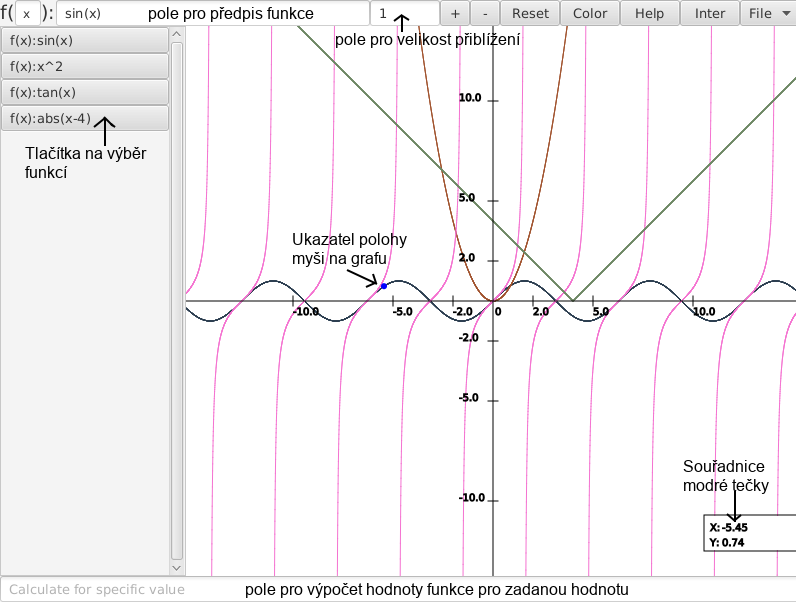
\includegraphics[height=10cm]{../img/layout.png}
	\caption{Okno programu}
\end{figure}
Ovládání programu je relativně jednoduché.
Uživatel nejprve zadá proměnou do malého vstupního pole v~horním rohu, tou může být jakékoliv písmeno v~anglické abecedě, až na písmeno e, to slouží jako konstanta $e$, $e \approx 2.71$.
Dále uživatel zadá předpis samotné funkce do pole napravo od pole s~proměnou.
Předpis je zapsán pomocí standardního matematického zápisu, program podporuje i~některé matematické funkce, jedná se o~absolutní hodnotu, goniometrické funkce a~jejich opaky, funkce ceil, floor, sqrt a~nalezení menšího, či většího čísla ze dvou zadaných.
Je také možné použití konstant, těmi jsou $e, \pi, \phi$.
Nutno upozornit, že desetinná čísla jsou oddělena desetinou tečkou, nikoliv čárkou.
Pro vykreslení grafu stačí v~poli s~předpisem stisknout klávesu enter.
Před vykreslením, je ještě možnost nastavit barvu grafu funkce, ty se standardně nastavují dle předdefinovaných barev, pomocí tlačítka color si však uživatel může nastavit vlastní.
Barvu grafu lze po vykreslení jednoduše změní tím, že nechá vykreslit graf znovu s~jinou barvou.

Pokud bude uživatel přejíždět myší po plátně, tak na grafu se bude zobrazovat malá modrá tečka, její pozice je zobrazena ve spodním pravém rohu.
Lze také vypočítal hodnotu grafu pro určenou hodnotu neznámé, k~tomu slouží pole vespodu okna.
Mezi grafy, pro které se počítají hodnoty se přechází prostřednictvím, menu na levé strany obrazovky, do něhož se graf automaticky po zobrazení přidá, pokud menu obsahuje mnoho grafů, stačí použít posuvník a~stáhnout menu dolů.
Vykreslené grafy si uživatel může libovolně oddalovat a přibližovat, za pomocí scrollování na myši, zadávacího pole na horní liště, či tlačítek + a -, jež najde také na horní liště.
Maximální hodnota je přiblížení je 1 a~minimální 100.

Pokud si uživatel chce nakreslené grafy uchovat do příštího spuštění programu (program nic dlouhodobě neukládá do paměti), může z~menu File vybrat možnost Export.
Ta uživateli zobrazí průzkumník souborů, kde vybere, či vytvoří soubor do něhož se uloží informace o~vykresleních grafech.
Po další spuštění pak jednoduše zvolí v~menu File položkou Import a~vybere soubor, který před ukončením nechal vytvořit.
Pokud uživatel chce uložit vykreslené grafy jen jako obrázek, pak z~menu File vybere možnost Save Img.

Program má ještě možnost najít souřadnice průsečíků dvou grafů, které leží v~rozmezí maxima a~minima osy~x na plátně.
K tomu slouží tlačítko Inter (z anglického intersection), po jeho stisknutí pomocí menu nakreslených funkcí vybereme jednu z~funkcí, jako druhá funkce slouží ta, která byla aktuálně vybraná před přechodem do Inter módu.
Pokud uživatel vybere funkci, která je stejná jako funkce, která byla vybrána před přechodem do módu Inter, tak program zobrazí body kde funkce protíná osu~X.
Pro vrácení zpět do módu vykreslování je třeba stisknout tlačítko Back.

Nápovědu k~použití programu lze zobrazit lehce pomocí tlačítka Help, nutno zdůraznit, že stejně jako zbytek programu je v~jazyce anglickém.

\section{Programová stránka UI}

Program je psaný za pomocí JavaFX konkrétněji v~JavaFXML, jedná se proto o~GUI aplikaci vykreslující se v~okně.
K jejímu spuštění je tak k~zapotřebí kromě Javy i~nějaký systém pro vytváření oken jako X.org.
Pevné rozložení prvků na obrazovce je uloženo v~souboru s~příponou .fxml, dynamické prvky UI jsou pak definovány v~samotném programu a~to ve dvou případech.
Zaprvé se jedná o~tlačítka na postranní liště.
Zadruhé je jím mód pro zobrazení souřadnic průsečíků dvou grafů, jelikož se jedná jen o~jeden prvek UI, bylo zbytečné vytvářet novou scénu s~vlastním .fxml souborem.
Samotná plocha na vykreslování grafů, se také mění dynamicky, to je něco co Canvas v~základu neumí, požadovaného výsledku bylo dosaženo použitím objektu Pane.
Jeho velikost se již dynamiky mění s~rozměry okna, na Pane se dále zavolá metoda getChildrem kde se mu přidá Canvas.
Tomu se pak svážou rozměry s~rozměry Pane a~přidají Listenery na rozměry okna, ty v~případě změny graf překreslí.
K~tomuto účelu slouží třída ResizableCanvas, ta se nachází v souboru FXMLDocumentControler.
Společně s~velikostí okna pro vykreslení se mění i~velikost polí na zadávání předpisu funkce a~výpočtu hodnoty funkce pro libovolnou hodnotu.
Poznámka autora: Třída ResizableCanvas byla převzata z mého předchozího projektu, ten jsem programoval na kroužku před nástupem na tuto školu, neuvádím proto citaci i~když kód je podobný s~tím co uvádí na internetu.

Základem rozložení programu je BorderPane, v~jeho horním kontejneru se nachází HBox.
Ten obsahuje většinu ovládacích prvků programu -- pole pro zadání proměnné (to má po stranách dva Labely s~texty f( a )=), pole pro zadání předpisu funkce ~pole zadání hodnoty přiblížení grafu.
Dále tlačítka na zmenšení/zvětšení přiblížení, zresetování programu do původního stavu, nastavení barvy grafu (před jeho vykreslením), zobrazení nápovědy, přejití do módu pro hledání průsečíků a~menu pro operace se soubory ‒ export do obrázku, export dat z~ParsedExpression do JSON a~import dat ze souboru JSON.
Ve středu BorderPane je Pane (se kterým je svázaný Canvas).
V~levém kontejneru se dále nachází ScrollPane, do kterého je zabalen VBox.
Na závěr ve spodním kontejneru se nachází TextField, pro výpočet hodnoty funkce pro danou hodnotu.
V~módu na zobrazení průsečíků se místo objektu Pane nastaví na střed TextArea, zároveň se také nastaví globální proměnná ovlivňující funkci tlačítek na vybrání funkce.
Ty tak místo nastavení proměnných do TextFieldů a kalkulátoru postfixových výrazů, zavolají funkci v PostFixExpressionCalculator.
Samozřejmě se také změní text tlačítka Inter na text Back, tlačítko potom složí k návratu do normálního módu.
Dle původního plánu by tlačítko Inter měnilo funkci tlačítek z~menu, ty by jim byly přiřazeny jakožto funkce lamba, z~toho ale sešlo, protože nejde měnit funkci tlačítka na funkci, která ještě nebyla definovaná, proto bylo také nutno přidat další globální proměnou.


\chapter{Backend}

\section{Postfixový kalkulátor}

\subsection{Dev log}

Nejtěžším problémem práce bylo vypočítání hodnoty funkce.
Java totiž, podobně jako většina hlavních programovacích jazyků, neumožňuje vypočítat hodnotu matematického výrazu, který je zadán v~podobě Stringu.

Prvotním plánem bylo použít objekt zvaný ScriptEngineManager, jemuž se přidá skrtiptovací engine, jako je třeba JavaScript a~ten již dokáže vypočítat hodnotu výrazu z~neznámé.
S~použitím ScriptEngineManageru by pak stačilo převést uživatelem zadaný výraz do zápisu s~voláním na knihovnu Math, čehož lze lehce dosáhnout pomocí jednoho cyklu a~podcyklu pokud obsahuje mocninu, či odmocninu, kde je potřeba najít základ a~mocnitele.
Toto řešení má ale dva hlavní problémy.
Zaprvé umožňuje spuštění JavaScriptového kódu, který zadá uživatel do pole pro předpis funkce, to sice není velký problém v~tomto případě, ale i~tak je lepší, aby uživatel neměl možnost spouštět příkazy tam kde být spuštěny nemají.
Větším problémem byla rychlost výpočtu hodnot funkce, trvalo několik sekund, než se vypočítaly hodnoty jedné funkce.
I~tak však program nebyl funkční, u~funkcí jako je tan, kde se na malém úseku přejde z~velkého čísla do malého čísla se nevykreslovaly velké úseky, a~nebylo možno vypočítat dostatek hodnot v~přijatelném čase.
Toto je problém, který se objevoval pořád během vývojového cyklu.
Použití ScriptEngineManageru tedy nepřicházelo v~úvahu, jako další možnost se naskytlo rekurzivně vypočítat rovnici sám.

U~této varianty byly dvě možnosti, a~to vytvořit objektovou reprezentaci funkce, či pokaždé vypočítat samotný String.
Objektová reprezentace vyžadovala udělat node pro každou specifickou část (znaménko, číslo, proměnná, funkce), pomocí nich pak vytvořit strom a~ten zespodu vždy vypočítat.
Toto řešení bylo velmi dlouhé a pochybně efektivní.
Způsob vypočítat pokaždé String byl zase pomalý, protože se musel string vždy zpracovávat.
Kód byl také velmi nepřehledný a~značně inspirovaný internetem.

Jako další možnost se jevilo použití jiného matematického zápisu než je ten standardní, infixový.
Ten by totiž umožňoval lehčí výpočet funkce, zatímco standardní zápis obsahuje složité konstrukce jako závorky, či přednost početních operací, tak například postfixový je nemá.
V~postfixové zápisu je tedy mnohem lehčí určit hodnotu výrazu.
Například příklad $(5+1)*(6-3)$, je v~postfixovém zápise $5 1 + 6 3 - *$, tento výraz již lze jednoduše vypočítat, za pomocí zásobníku, kam se budou ukládat čísla a~narazí li se na nějakou operaci, jednoduše si program za zásobníku vyhodí číslo/a provede na nich operaci.
Výsledek poté uloží zpět do zásobníku, nakonec v~zásobníku zůstane jen jedno číslo a~to je konečným výsledkem.
Způsob výpočtu přes postfix je navíc relativně rychlý, protože složitost výpočtu je pouhý O(n).

\subsection{Gramatika uživatelova zápisu}

Matematický zápis předpisu funkce se vesměs řídí standardními matematickými pravidly.
Desetinná čísla jsou však zapsána s~desetinou tečkou, aby byl zápis konzistentní se zbytkem programu, který je v angličtině.
Proměnou může být jakékoliv písmeno z~anglické abecedy, až na písmeno e.
To a~řetězce phi a~pi jsou vyhrazeny pro matematické konstanty.
Standardní operace se zapisují pomocí symbolů +, -, *, /.
Předpis může či nemusí obsahovat mezery.
K~mocnině slouží značka \string^, pro zapsání odmocniny se do závorky zapíše převrácená hodnota mocniny, např. $\sqrt{3}$ = 3\string^(1/2).
Funkce jsou napsané standardně a~jejich argumenty jsou v závorkách, např sin(x), tan(4).
Absolutní hodnoty se zapisují pomocí funkce abs, znak | nebude zpracován a~vyústí v chybovou hlášku.
Program podporuje dvě funkce (max a min), které potřebují dva argumenty, v~jejich případě budou argumenty odděleny čárkou.
Chce li uživatel použít záporné číslo např $x*(-3)$, tak číslo musí být v~závorkách.
Jen v~případě, že se jedná o~první znak zápisu může být bez závorek.
Bude li číslo před závorkou, nebo před funkcí, program vyhodí chybovou hlášku, závorka nebude vynásobena.

\subsection{Počítání s postfixem}

\subsubsection{Převedení do postfixového zápisu}

Na výpočet s~postfixovým zápisem je potřeba nejprve převést uživatelem zadaný infixový String do postfixového Listu (s listem se lehčeji zachází).
K~tomuto účelu slouží algoritmus Shunting-yard vymyšlený Edsgerem Dijkstrou \cite{EWD61}.
Ten funguje na jednoduchém principu jednoho zásobníku a~listu.
Nalezne li algoritmus číslo, neznámou, či proměnou přidá ji na konec listu.
Nalezna li operaci, tak začne procházet zásobník a přidají se do výsledného liste všechny operace, které mají větší, nebo rovnou přednost.
Takto bude čísla přidávat, a~z~zásobníku odstraňovat, dokud nenajde číslo s~menší předností, levou závorku, funkci, nebo nedojde na konec zásobníku.
Po skončení přidávání operaci přidá do zásobníku.
Nalezne li levou závorku, či funkci jednoduše ji přidá do zásobníku.
Nalezne li pravou závorku ze zásobníku postupně přidá vše dokud nenalezna závorku levou, tu smaže a~nepřidá do listu.
Nakonec postupně přidá celý zásobník na konec listu.
V~programu je tento algoritmus implementován pomocí tří tříd.

První je třída Precedence, ta obsahuje Enumy s~informacemi o~přednosti početních operací.
Ta má jen jednu metodu~s switch case, ta vrátí početní hodnotu operace podle zadaného Stringu.

Druhou třídou je OperatorStack, ta reprezentuje zásobník s~početními operacemi.
Obsahuje metody na standardní obsluhu zásobníku, přidání operace, funkce, metodu k~zavolání při nalezení závorky.
Zároveň může zobrazit Alert, pokud nebudou závorky v~páru.

Třetí a~hlavní složkou je třída PostfixExpressionCalc.
O~převedení do postfixu se stará metoda parse, ta je automaticky zavolána konstruktorem, konkrétně tím, který jako argument bere dva Stringy.
Metoda funguje na jednoduchém principu, kdy postupně prochází String a~hledá změny ve znacích, proto musí na začátku ke Stringu přičíst mezeru.
U~změn si vždy pamatuje indexy a~pomocí nich String dělí na substringy.
Těmi už jsou samotná čísla, konstanty, funkce.
Jeli řetězec číslo jednoduše ho přidá do Listu, obsahuje li znaky, zjistí zda se jedná o~proměnou, konstantu či funkci.
Při každé iteraci proběhne ještě switch case, který se řídí aktuálním charakterem, ten přidává operace +, -, *, / do zásobníku a~zajistí správné zpracování závorek a~čárky.
U~závorek zkontroluje zda je mezi nimi jen jedno číslo či neznámá, pokud ano, tak obsah mezi závorkami přidá do výsledného listu.
Na~závěr metoda vyprázdní zásobník s operacemi do listu.
Dojde li někde během převádění k~chybě (uživatelův vstup je v~rozporu se stanovenou gramatikou), tak program vytvoří okno s~upozorněním a~nastaví proměnou isExpressionCalculable na false.
Program pak ví, že nemá smysl se snažit příklad vypočítat.
Po skončení se zavolá metoda setUpRecognitionArray, ta nastaví pole, které obsahuje informace o~typu jednotlivých prvků postfixového zápisu, zda se jedná o~číslo, proměnou, atd.
V~praxi to vede ke zrychlení výpočtu, neb není potřeba při každém výpočtu zjišťovat typ prvku.

\subsubsection{Výpočet postfixového zápisu}

K~výpočtu postfixového zápisu slouží metoda evaluateExpression.
Výpočet je založen na jednom cyklu, který postupně prochází pole a~pomocí switche buďto přidá do zásobníku, nebo si z~zásobníku vezme prvky a~provede na nich operaci.
Zároveň během přidávání do zásobníku se za neznámou dosadí číslo, které metoda dostane v~argumentu.
Pokud najde funkci, kterou nezná vytvoří Alert a~nastaví proměnou isExpressionCalculable na false.
Pokud dojde k~takové chybě či jiné chybě během výpočtu, program vrátí Double.NaN.

\subsubsection{Hledání průsečíků}

Třída PostfixExpressionCalc obsahuje také metodu na nalezení průsečíků.
Ta funguje na relativně jednoduchém principu, metoda dostane jako argument druhou rovnici a~proměnou, kterou používá.
Pokud je proměnná jiná než, kterou používá funkce, která je aktuálně nastavená v~PostFixExpressionCalc, tak proběhne cyklus, který proměnné srovná.
Rovnice poté od sebe odečte, v~postfixovém zápisu je nejprve třeba přidat prvky druhé rovnice, až potom přidat znaménko mínus.
Po těchto úpravách můžeme již začít hledat pro jaké hodnoty se výraz rovná nule.
Na hledání těchto bodů je použita metoda zvaná bisection method \cite{Bisection-method}.
Ta je založená na principu, že pokud máme hodnotu funkce, která je kladná, a~hodnotu funkce, která je záporná, nutně se mezi nimi nachází průsečík s nulou.
Nejprve tedy program hrubě počítá hodnoty funkce a~najde li nějaké zlomové hodnoty, kde se mění znaménko, pomocí binary search nalezne přesný bod.
Program, hledá jen v~rozmezí osy~x, která je právě zobrazená na grafu.

Je pravda, že jiné algoritmy na řešení rovnic sice najdou řešení rovnic i~bez předem zadaného rozmezí, ty však často vyžadují derivaci funkce.
Vytváření derivací se však prvky jako min a~max značně komplikuje.
Navíc mnohé z~nich udají jen jeden výsledek rovnice.
Proto byla použita tato metoda, ačkoliv se jedná neefektivní řešení.
Co se týče rychlosti se však, díky jinak rychlému počítání rovnice, uživatel nemusí na výsledek dlouho čekat.
Metoda po skončení vrátí List s~body na souřadnici~x, kde dochází k~průniku.

Existují také vstupy pro které nemusí hrubé prohledávání najít zlomové body, tyto možnosti program neřeší. Příkladem může být f(x)=$x^2$ - 0.000 001.

\section{Controller k~FXML souboru}

\subsection{Inicizlizace programu}

O~samotné řízení programu se stará třída FXMLDocumentController.
Scénu a~Stage však nejdříve vytvoří třída GraphDraw, ta taky zavolá metodu setStage v~FXMLDocumentConroller, která se postará o~inicializaci UI, aby byl program připraven pro uživatelův vstup.
V metodě se vytvoří objekt ResizableCanvas, a~nastaví se globální proměnné jako je GraphicsContext2D, či CustomColorDialog.
Před skončením se zavolají metody drawScale a~drawMouseBox, které na plátno nakreslí osy a~ohraničení pro zobrazení pozice modrého bodu.
Je sporná užitelnost jejich použití, záleží na tom, jak který desktop, či window manager zachází s~novými okny.
Například v~případě window manageru i3wm se velikost okna několikrát změní ještě před tím, než se inicializuje GraphicsContext, což vede k~nullPointerExeption (všechny metody s~vykreslováním jsou proti ní chráněni), ale také už zavolají překreslení Listenery v~ResizableCanvas, čili se ohrádka a~osy vykreslí několikrát.
Vykreslování se obecně chová zvláštně v~této fázi, varianta uvedená v~programu však funguje.

\subsection{Metody sloužící k~vykreslování na Canvas}

Třída obsahuje celkem 8 metod, které vykreslují na Canvas, či volají metody vykreslující na Canvas.
Nejméně zajímavou z~nich je metoda drawMouseBox, ta se stará čistě o~vykreslení malého okénka pro zobrazení pozice modrého bodu.
Je však samostatná kvůli přehlednosti kódu a~navíc ji volá metoda (spíše lambda funkce) mouseMovedInCanas.
Ta bude popsána o~něco později.
Další metodu je metoda drawScale, ta se stará o~vykreslení os a~jejich popisků.
Měřítko osy je dáno hodnotou zoom, ta je v~rozmezí od 19 do 119.
Hraniční hodnoty jsou způsobeny funkcemi jako je tan, s~tímto měřítkem na fullhd monitoru nebude chybět kus jejich grafu.
Když se měřítko nastavovalo automaticky, aby se tomuto nedostatku předešlo, bylo zobrazování nepřehledné, proto je v~konečné verzi omezené těmito hodnotami.
I~přesto, že funkce např. f(x)=$tan(x)/100$, nebude vykreslena správně.
Metoda DrawScale také uloží obrázek s aktuálním stavem Canvasu do proměnné, metoda je totiž vždy volána před metodou drawMouseBox, jedná se tedy o~stav kdy jsou na plátně jen grafy funkcí a~osy.
Obrázek je pak používán lamba funkcí mouseMovedInCavas, ta vždy na plátno nakreslí obrázek grafů na něj modrou tečku, ta se tak pohybuje plynule s~pohybem myši, neboť se vždy nemusí překreslovat všechny grafy.
Metoda reDrawFunctions pomocí cyklu prochází vše uložené v~ParsedExpressions a~každý graf nakreslí, volají ji metody menuImportAction, update a drawGrahAction.
O~samotné vykreslení grafu se stará metoda drawToCanas, ta dostane jako argument List obsahující Point2D, ty projde a~spojí je čarami.

\subsubsection{Metoda drawGraphAction}

Tato metoda je volána vždy po zmáčknutí klávesy v~poli pro předpis funkce, její obsah se však vykoná jen pokud je zmáčknuta klávesa enter.
Pokud je stisknuta klávesa enter, vytvoří metoda objekt PostfixExpressionCalc a~jako argumenty do konstruktoru dá infixový předpis funkce a~její proměnou.
Poté provede jeden kontrolní výpočet, zdaří li se uloží si do proměnné kopii postfixového předpisu.
Než proběhne vykreslení zkontroluje zda uživatel změnil barvu funkce, jestli ne tak nastaví jednu z~předdefinovaných barev.
Není li funkce uložená v~ParsedExpression tak se uloží, pokud byla změněna barva, tak se přepíše na novou hodnotu.
Zároveň se vytvoří tlačítko v~HBoxu vlevo na vybrání funkce.
Poté se pomocí metody reDrawFunction zobrazí se samotný graf.

\subsection{Třída ParsedExpressions}
Třída ParsedExpression slouží k~uchování funkcí, které lze nakreslit.
Parametry funkcí jsou uloženy ve 4 Listech, ty si pamatují infixový zápis, postfixový zápis, barvy grafu a~proměnou.
Na obsluhu obsahuje standardní metody, jako jsou getry~a setry.
Obsahuje i~metody na generování a~psaní do souboru -- metody importFromJSON a~exportToJSON.
Metoda pro exportování funguje na primitivním principu -- postupně prochází všechny Listy a~data z~nich zapisuje do JSON, z~toho důvodu ani nebyly použity nástroje z~knihovny json.
Struktura souboru je jednoduchá, obsahuje pole functions, v~něm jsou postupně vypsané funkce.
\begin{lstlisting}[caption={Příklad JSON souboru},captionpos=b]
{
	"functions":[
		{
			"infix":"sin(x)",
			"postfix":"x, sin",
			"color":"#2c3e50",
			"variable":"x"
		},
		{
			"infix":"abs(abs(x+1)-abs(x-2))",
			"postfix":"x, 1, +, abs, x, 2, -, abs, -, abs",
			"color":"#a0522d",
			"variable":"x"
		}
	]
}

\end{lstlisting}

Při čtení JSON je použita knihovna json \cite{Stleary15}.
Obsah celého souboru se nejprve načte do jednoho Stringu.
Ten je použit jako argument v~konstruktoru pro JSONObject.
Z~toho se poté dostane pole functions, to se uloží do JSONArray.
Program pak pole prochází zpracuje jejich vstup (postfix převede na List, k~barvě přidá 0x a ff, atd.), provede kontrolní výpočet a~pokud vše proběhne správně funkci přidá do Listů.
Metoda vrátí true, jestliže něco bylo přidané do Listů.
FXMLDocumentController v~tomto případě totiž překreslí grafy.

Předpokládá se, že velikost souboru je malá, proto je předán JSON do JSONObject v~podobě Stringu a~na čtení souborů není vytvořeno není vlákno.

Ukládání rovnic by šlo řešit za pomocí ObservableList a~objektu, který by reprezentoval jednu funkci.
Třída FXMLDocumentControler, však potom musela obsahovat metody pro exportování a importování ze souboru.
Tím se stávala (dle názoru autora) nepřehlednou.
Byl proto použit způsob, kde jedna třída obsahuje čtyři Listy.

\chapter*{Závěr}
\addcontentsline{toc}{chapter}{Závěr}
Dle mého názoru byly cíle práce naplněny.
Ve své finální podobě program kromě vykreslování grafů dokáže grafy i~exportovat.
Zároveň je také možno hledat dvou průsečíky grafů.
Jediným výrazným nedostatkem je možné chybné zobrazení u~funkcí jako je tan, zde, ale nevím jak problém vyřešit, protože nejde předpokládat, že graf půjde automaticky do nekonečna u\,všech takových případů.
Ideální řešení by nejspíš vyžadovalo komplexnější analýzy předpisu funkce, což je něco co je nad mé schopnosti.
Samozřejmě je to však jedna složka která je otevřená k~dalšímu rozvinutí a~vylepšení.
Celá práce je dostupná na stránce GitHub pod licencí WTFPL (URL: \url{https://github.com/havrak/GraphDraw}).


%%% Seznam použité literatury (bibliografie)
%%%
%%% Pro vytváření bibliografie používáme bibTeX. Ten zpracovává
%%% citace v textu (např. makro \cite{...}) a vyhledává k nim literaturu
%%% v souboru literatura.bib.
%%%
%%% Příkaz \bibliographystyle určuje, jakým stylem budou citovány odkazy
%%% v textu. V závorce je název zvoleného souboru .bst. Styly plainnat
%%% a unsrt jsou standardní součástí latexových distribucí. Styl czplainnat
%%% je dodáván s touto šablonou a bibTeX ho hledá v aktuálním adresáři.

\bibliographystyle{czplainnat}    %% Autor (rok) s českými spojkami
% \bibliographystyle{plainnat}    %% Autor (rok) s anglickými spojkami
\bibliographystyle{unsrt}       %% [číslo]

\renewcommand{\bibname}{Seznam použité literatury}

%%% Vytvoření seznamu literatury. Pozor, pokud jste necitovali ani jednu
%%% položku, seznam se automaticky vynechá.

\bibliography{literatura}

%%% Kdybyste chtěli bibliografii vytvářet ručně (bez bibTeXu), lze to udělat
%%% následovně. V takovém případě se řiďte normou ISO 690 a zvyklostmi v oboru.

% \begin{thebibliography}{99}
%
% \bibitem{lamport94}
%   {\sc Lamport,} Leslie.
%   \emph{\LaTeX: A Document Preparation System}.
%   2. vydání.
%   Massachusetts: Addison Wesley, 1994.
%   ISBN 0-201-52983-1.
%
% \end{thebibliography}


\openright
\end{document}
